\section{Experiments}
\label{sec:exp}

\begin{table}[t]
\small\centering\setlength{\tabcolsep}{3pt}
\begin{tabular}{l | c | g | g g g g }
\toprule
\rowcolor{white} \textbf{ImageNet 256$\times$256} & Latent Shape & Autoencoder & rFID $\downarrow$ & PSNR $\uparrow$ & SSIM $\uparrow$ & LPIPS $\downarrow$ \\
\midrule
\rowcolor{white} \multirow{2}{*}{f32c32} & \multirow{2}{*}{8$\times$8$\times$32} 
 & SD-VAE \tablecite{rombach2022high} & 2.64 & 22.13 & 0.59 & 0.117 \\
 & & \modelshort                      & \textbf{0.69} & \textbf{23.85} & \textbf{0.66} & \textbf{0.082} \\
\midrule
\rowcolor{white} \multirow{2}{*}{f64c128} & \multirow{2}{*}{4$\times$4$\times$128}
 & SD-VAE \tablecite{rombach2022high} & 26.65 & 18.07 & 0.41 & 0.283 \\
 & & \modelshort                      & \textbf{0.81} & \textbf{23.60} & \textbf{0.65} & \textbf{0.087} \\
\bottomrule
\toprule
\rowcolor{white} \textbf{ImageNet 512$\times$512} & Latent Shape & Autoencoder & rFID $\downarrow$ & PSNR $\uparrow$ & SSIM $\uparrow$ & LPIPS $\downarrow$ \\
 \midrule
\rowcolor{white} \multirow{2}{*}{f64c128} & \multirow{2}{*}{8$\times$8$\times$128}
 & SD-VAE \tablecite{rombach2022high} & 16.84 & 19.49 & 0.48 & 0.282 \\
 & & \modelshort                      & \textbf{0.22} & \textbf{26.15} & \textbf{0.71} & \textbf{0.080} \\
\midrule
\rowcolor{white} \multirow{2}{*}{f128c512} & \multirow{2}{*}{4$\times$4$\times$512}
 & SD-VAE \tablecite{rombach2022high} & 100.74 & 15.90 & 0.40 & 0.531 \\
 & & \modelshort                      & \textbf{0.23} & \textbf{25.73} & \textbf{0.70} & \textbf{0.084} \\
\bottomrule
\toprule
\rowcolor{white} \textbf{FFHQ 1024$\times$1024} & Latent Shape & Autoencoder & rFID $\downarrow$ & PSNR $\uparrow$ & SSIM $\uparrow$ & LPIPS $\downarrow$ \\
\midrule
\rowcolor{white} \multirow{2}{*}{f64c128} & \multirow{2}{*}{16$\times$16$\times$128}
 & SD-VAE \tablecite{rombach2022high} & 6.62 & 24.55 & 0.68 & 0.237 \\
 & & \modelshort                      & \textbf{0.23} & \textbf{31.04} & \textbf{0.83} & \textbf{0.061} \\
 \midrule
\rowcolor{white} \multirow{2}{*}{f128c512} & \multirow{2}{*}{8$\times$8$\times$512}
 & SD-VAE \tablecite{rombach2022high} & 179.71 & 18.11 & 0.63 & 0.585 \\
 & & \modelshort                      &  \textbf{0.41} & \textbf{31.18} & \textbf{0.83} & \textbf{0.062} \\
\bottomrule
\toprule
\rowcolor{white} \textbf{MapillaryVistas 2048$\times$2048} & Latent Shape & Autoencoder & rFID $\downarrow$ & PSNR $\uparrow$ & SSIM $\uparrow$ & LPIPS $\downarrow$ \\ 
 \midrule
\rowcolor{white} \multirow{2}{*}{f64c128} & \multirow{2}{*}{32$\times$32$\times$128}
 & SD-VAE \tablecite{rombach2022high} & 7.55 & 22.37 & 0.68 & 0.262 \\
 & & \modelshort                      & \textbf{0.36} & \textbf{29.57} & \textbf{0.84} & \textbf{0.075} \\
 \midrule
\rowcolor{white} \multirow{2}{*}{f128c512} & \multirow{2}{*}{16$\times$16$\times$512} 
 & SD-VAE \tablecite{rombach2022high} & 152.09 & 17.82 & 0.67 & 0.594 \\
 & & \modelshort                      &  \textbf{0.38} & \textbf{29.70} & \textbf{0.84} & \textbf{0.074} \\
\bottomrule
\end{tabular}
\vspace{-5pt}
\caption{\textbf{Image Reconstruction Results.}}
\vspace{-10pt}
\label{tab:ae_main}
\end{table}

\subsection{Setups}

\paragraph{Implementation Details.} We use a mixture of datasets to train autoencoders (baselines and \modelshort), containing ImageNet \citep{deng2009imagenet}, SAM \citep{kirillov2023segment}, MapillaryVistas \citep{neuhold2017mapillary}, and FFHQ \citep{karras2019style}. For ImageNet experiments, we exclusively use the ImageNet training split to train autoencoders and diffusion models. The model architecture is similar to SD-VAE \citep{rombach2022high} except for our new designs discussed in Section~\ref{sec:main_model}. In addition, we use the original autoencoders instead of the variational autoencoders for our models, as they perform the same in our experiments and the original autoencoders are simpler. We also replace transformer blocks with EfficientViT blocks \citep{cai2023efficientvit} to make autoencoders more friendly for handling high-resolution images while maintaining similar accuracy. 

For image generation experiments, we apply autoencoders to diffusion transformer models including DiT \citep{peebles2023scalable} and UViT \citep{bao2023all}. We follow the same training settings as the original papers. 
We consider three settings with different resolutions, including ImageNet \citep{deng2009imagenet} for $512 \times 512$ generation, FFHQ \citep{karras2019style} and MJHQ \citep{li2024playground} for $1024 \times 1024$ generation, and MapillaryVistas \citep{neuhold2017mapillary} for $2048 \times 2048$ generation. 

\begin{table}[t]
\small\centering\setlength{\tabcolsep}{2pt}
\begin{tabular}{l | g | g | g g | g | g | g g }
\toprule
\rowcolor{white} Diffusion & & Patch & \multicolumn{2}{c|}{Throughput (image/s) $\uparrow$} & Latency & Memory & \multicolumn{2}{c}{FID $\downarrow$} \\
\rowcolor{white} Model & \multirow{-2}{*}{Autoencoder} & Size & Training & Inference & (ms) $\downarrow$ & (GB) $\downarrow$ & w/o CFG & w/ CFG \\
\midrule
\rowcolor{white} & SD3-VAE-f8 \tablecite{esser2024scaling}                   & 2 &  352 &  2984 & 3.8 & 13.8 & 164.34 & 143.82 \\
\rowcolor{white} & Flux-VAE-f8 \tablecite{flux2024}                          & 2 &  352 &  2984 & 3.8 & 13.8 & 106.07 & 84.73 \\
\cmidrule{2-9}
\rowcolor{white} & SDXL-VAE-f8 \tablecite{podell2023sdxl}                    & 2 &  352 &  2991 & 3.8 & 13.8 & 51.03 & 26.38 \\
\rowcolor{white} & Asym-VAE-f8 \tablecite{zhu2023designing}                  & 2 &  352 &  2991 & 3.8 & 13.8 & 51.96 & 24.57 \\
\rowcolor{white} & SD-VAE-f8 \tablecite{rombach2022high}                     & 2 &  352 &  2991 & 3.8 & 13.8 & 51.96 & 24.57 \\
\rowcolor{white} & SD-VAE-f16 \tablecite{rombach2022high}                    & 2 & 1550 & 12881 & 1.3 &  4.0 & 76.86 & 44.22 \\
\rowcolor{white} & SD-VAE-f32 \tablecite{rombach2022high}                    & 1 & 1551 & 12883 & 1.3 &  4.0 & 70.23 & 38.63 \\
\cmidrule{2-9}
& \modelshort-f32                                                            & 1 & 1553 & 12850 & 1.3 &  4.0 & \textbf{46.12} & \textbf{18.08} \\ 
& \modelshort-f64                                                            & 1 & \textbf{6295} & \textbf{53774} & \textbf{0.7} & \textbf{1.5} & 67.30 & 35.96 \\
\multirow{-11}{*}{UViT-S \tablecite{bao2023all}} & \:\:\modelshort-f64$^\dag$ & 1 & \textbf{6295} & \textbf{53774} & \textbf{0.7} & \textbf{1.5} & 61.84 & 30.63 \\
\midrule
\midrule
\rowcolor{white} & Flux-VAE-f8 \tablecite{flux2024}                          & 2 &   54 &  416 & 31.7 & 56.3 & 27.35 & 8.72 \\
\cmidrule{2-9}
\rowcolor{white} & Asym-VAE-f8 \tablecite{zhu2023designing}                  & 2 &   54 &  424 & 31.7 & 56.2 & 11.55 & 2.95 \\
\rowcolor{white} &  SD-VAE-f8 \tablecite{rombach2022high}                    & 2 &   54 &  424 & 31.7 & 56.2 & 12.03 & 3.04 \\
\cmidrule{2-9}
& \modelshort-f32                                                            & 1 &  \textbf{241} &  \textbf{2016} & \textbf{7.8} & \textbf{20.9} &  9.56 & 2.84 \\
\multirow{-5}{*}{DiT-XL \tablecite{peebles2023scalable}} 
& \:\:\modelshort-f32$^\ddag$                                                    & 1 &  \textbf{241} &  \textbf{2016} & \textbf{7.8} & \textbf{20.9} &  \textbf{6.88} & \textbf{2.41} \\


\midrule
\midrule
\rowcolor{white} & Flux-VAE-f8 \tablecite{flux2024}                          & 2 &  55 &  349 & 30.4 & 54.2 & 30.91 & 12.63 \\
\cmidrule{2-9}
\rowcolor{white} & Asym-VAE-f8 \tablecite{zhu2023designing}                  & 2 &  55 &  351 & 30.3 & 54.1 & 11.36 &  3.51 \\
\rowcolor{white}  & SD-VAE-f8 \tablecite{rombach2022high}                    & 2 &   \,\,55\,\,\tikzmark{uvit_h_f8p2:a1} &   \,\,351\,\,\tikzmark{uvit_h_f8p2:a2} & 30.3 & 54.1 & 11.04 & \,\,3.55\,\,\tikzmark{uvit_h_f8p2:a3} \\
\cmidrule{2-9}
& \modelshort-f32                                                            & 1 &  247 &  1622 &  8.2 & 18.6 &  \textbf{9.83} & \textbf{2.53} \\
& \modelshort-f64                                                            & 1 & \,\,\textbf{984}\,\,\tikzmark{uvit_h_f64p1:a1} &  \,\,\textbf{6706}\,\,\tikzmark{uvit_h_f64p1:a2} & \textbf{3.5} & \textbf{10.6} & 13.96 & \,\,3.01\,\,\tikzmark{uvit_h_f64p1:a3} \\
\multirow{-6}{*}{UViT-H \tablecite{bao2023all}} & \:\:\modelshort-f64$^\dag$ & 1 & \textbf{984} &  \textbf{6706} & \textbf{3.5} & \textbf{10.6} & 12.26 & 2.66 \\

\midrule
\midrule
\rowcolor{white} & Asym-VAE-f8 \tablecite{zhu2023designing}                   & 2 &  27 & 157 & 74.8 & OOM & 9.87 & 3.62 \\
\rowcolor{white}  & SD-VAE-f8 \tablecite{rombach2022high}                     & 2 &  27 & 157 & 74.8 & OOM & 9.73 & 3.57 \\
\cmidrule{2-9}
& \modelshort-f32                                                             & 1 & 112 & 665 & 19.7 & 42.0 & 8.13 & 2.30 \\
& \modelshort-f64                                                             & 1 & \textbf{450} & \textbf{2733} & \textbf{8.6} & \textbf{30.2} & 7.78 & 2.47 \\
\multirow{-5}{*}{UViT-2B \tablecite{bao2023all}} & \:\:\modelshort-f64$^\dag$ & 1 & \textbf{450} & \textbf{2733} & \textbf{8.6} & \textbf{30.2} & \textbf{6.50} & \textbf{2.25} \\

\bottomrule
\end{tabular}

\begin{tikzpicture}[overlay, remember picture, shorten >=.5pt, shorten <=.5pt, transform canvas={yshift=.25\baselineskip}]

\draw [->, red] ({pic cs:uvit_h_f8p2:a1}) [bend left] to node [below right] (uvit_h_f8p2:t1) {\hspace{-2pt}\scriptsize \textbf{17.9$\times$}} ({pic cs:uvit_h_f64p1:a1});

\draw [->, red] ({pic cs:uvit_h_f8p2:a2}) [bend left] to node [below right] (uvit_h_f8p2:t2) {\hspace{-2pt}\scriptsize \textbf{19.1$\times$}} ({pic cs:uvit_h_f64p1:a2});

\draw [->, red] ({pic cs:uvit_h_f8p2:a3}) [bend left] to node [below right] (uvit_h_f8p2:t3) {\hspace{-2pt}\scriptsize \textbf{-0.54}} ({pic cs:uvit_h_f64p1:a3});

\end{tikzpicture}
\vspace{-5pt}
\caption{\textbf{Class-Conditional Image Generation Results on ImageNet 512$\times$512.} $^\dag$ represents the model is trained for 4$\times$ training iterations (i.e., 500K $\rightarrow$ 2,000K iterations). $^\ddag$ represents the model is trained with 4$\times$ batch size (i.e., 256 $\rightarrow$ 1024).}
\label{tab:diffusion_imagenet_main}
\end{table}


\begin{table}[t]
\small\centering\setlength{\tabcolsep}{2pt}
\begin{tabular}{l | g | g | g g | g | g | g g }
\toprule
\rowcolor{white} Diffusion & & Patch & \multicolumn{2}{c|}{Throughput (image/s) $\uparrow$} & Latency & Memory & \multicolumn{2}{c}{MJHQ 512$\times$512} \\
\rowcolor{white} Model & \multirow{-2}{*}{Autoencoder} & Size & Training & Inference & (ms) $\downarrow$ & (GB) $\downarrow$ & FID $\downarrow$ & CLIP Score $\uparrow$ \\
\midrule
\rowcolor{white} & SD-VAE-f8 \tablecite{rombach2022high} & 2 & 43 & 312 & 37.1 & 60.45 & 6.3 & 26.36 \\
\multirow{-2}{*}{PIXART-$\alpha$ \tablecite{chenpixart}} 
& \modelshort-f32                                        & 1 & \textbf{173} & \textbf{1251} & \textbf{10.4} & \textbf{23.77} & \textbf{6.1} & \textbf{26.41} \\
\bottomrule
\end{tabular}
\vspace{-5pt}
\caption{\textbf{Text-to-Image Generation Results.}}
\vspace{-10pt}
\label{tab:diffusion_t2i_main}
\end{table}


\begin{figure}[t]
    \centering
    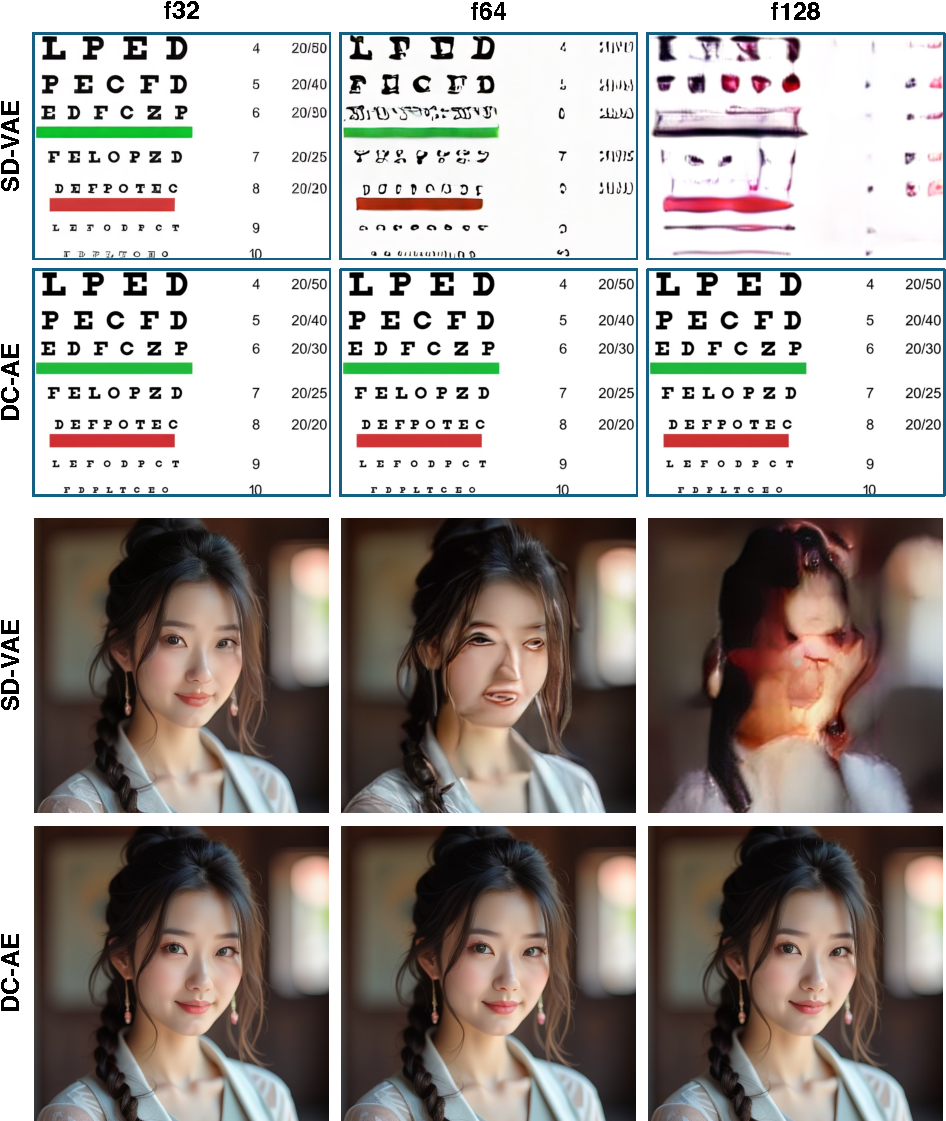
\includegraphics[width=0.95\linewidth]{figures/src/ae_visualization.pdf}
    \vspace{-10pt}
    \caption{\textbf{Autoencoder Image Reconstruction Samples.}}
    \vspace{-10pt}
    \label{fig:ae_visualization}
\end{figure}


\begin{figure}[t]
    \centering
    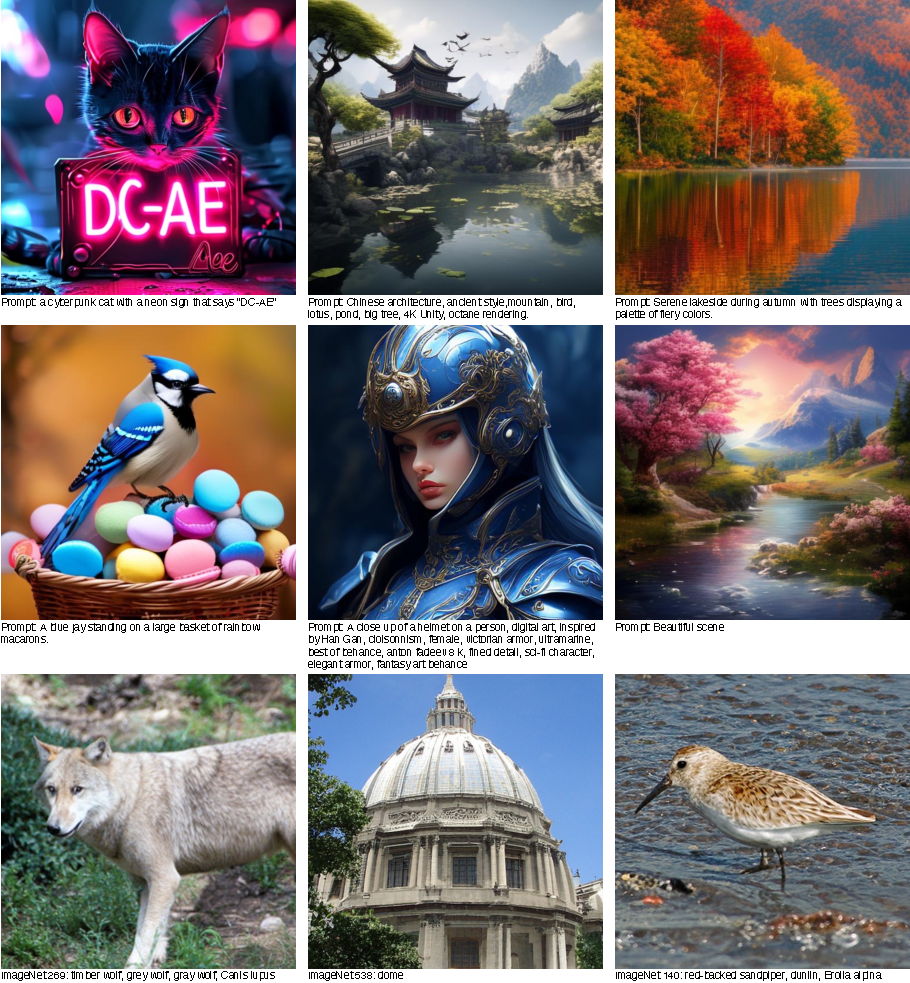
\includegraphics[width=1\linewidth]{figures/src/diffusion_visualization.pdf}
    \vspace{-15pt}
    \caption{\textbf{Images Generated by Diffusion Model using Our \modelshort.}}
    \vspace{-10pt}
    \label{fig:diffusion_visualization}
\end{figure}


\paragraph{Efficiency Profiling.} We profile the training and inference throughput on the H100 GPU with PyTorch and TensorRT respectively. The latency is measured on the 3090 GPU with batch size 2. The training memory is profiled using PyTorch, assuming a batch size of 256. We use fp16 for all cases. For simplicity, we assume the number of sampling steps is 1.

\subsection{Image Compression and Reconstruction}
Table~\ref{tab:ae_main} summarizes the results of \modelshort and SD-VAE \citep{rombach2022high} under various settings (f represents the spatial compression ratio and c denotes the number of latent channels). \modelshort provides significant reconstruction accuracy improvements than SD-VAE for all cases. For example, on ImageNet $512 \times 512$, \modelshort improves the rFID from 16.84 to 0.22 for the f64c128 autoencoder and 100.74 to 0.23 for the f128c512 autoencoder. 

In addition to the quantitative results, Figure~\ref{fig:ae_visualization} shows image reconstruction samples produced by SD-VAE and \modelshort. Reconstructed images by \modelshort demonstrate a better visual quality than SD-VAE's reconstructed images. In particular, for the f64 and f128 autoencoders,  \modelshort still maintains a good visual quality for small text and the human face. 

\subsection{Latent Diffusion Models}
We compare \modelshort with the widely used SD-VAE-f8 autoencoder \citep{rombach2022high} on various diffusion transformer models. For \modelshort, we always use a patch size of 1 (denoted as p1). For SD-VAE-f8, we follow the common setting and use a patch size of 2 or 4 (denoted as p2, p4). The results are summarized in Table~\ref{tab:diffusion_imagenet_main}, Table~\ref{tab:diffusion_hr_main}, and Table~\ref{tab:diffusion_t2i_main}. 

\vspace{-5pt}
\paragraph{ImageNet 512$\times$512.} As shown in Table~\ref{tab:diffusion_imagenet_main}, \modelshort-f32p1 consistently delivers better FID than SD-VAE-f8p2 on all diffusion transformer models. In addition, it has 4$\times$ fewer tokens than SD-VAE-f8p2, leading to 4.5$\times$ higher H100 training throughput and 4.8$\times$ higher H100 inference 
\begin{wrapfigure}{r}{0.35\textwidth}
  \vspace{-10pt}
  \begin{center}
    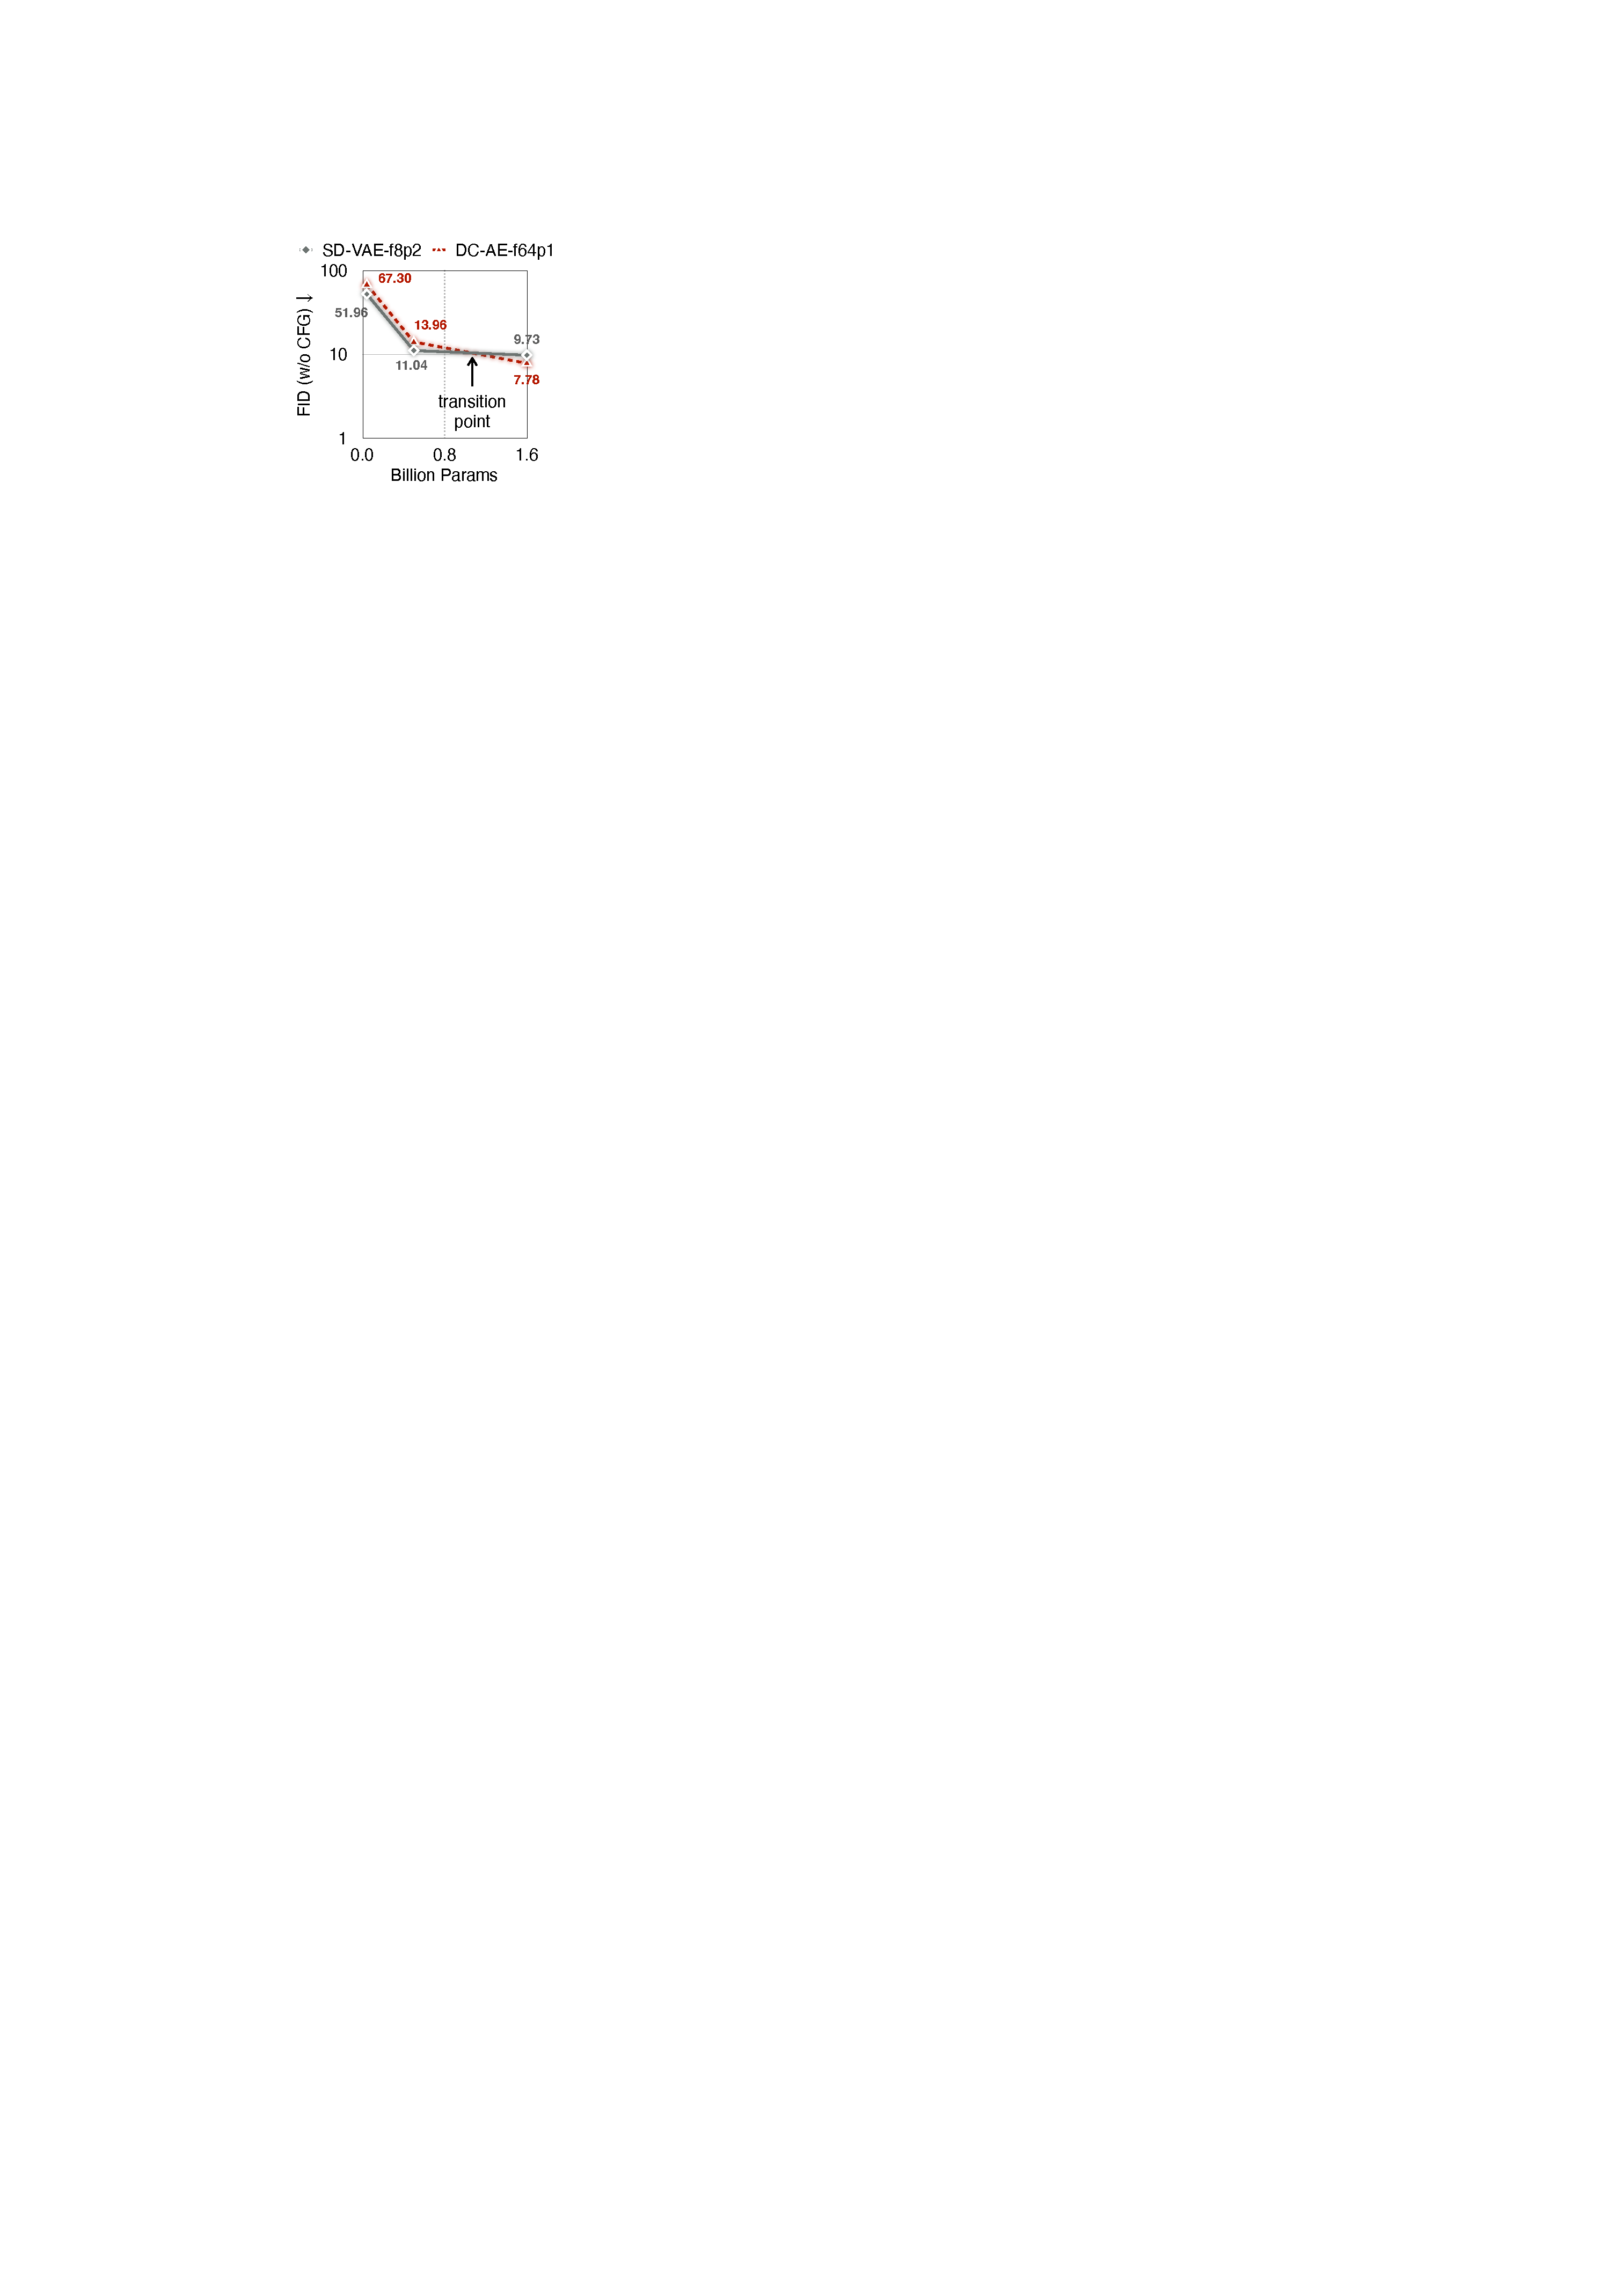
\includegraphics[width=0.35\textwidth]{figures/src/diffusion_scaling_up.pdf}
  \end{center}
  \vspace{-10pt}
  \caption{\textbf{Model Scaling Results on ImageNet 512$\times$512 with UViT.} \modelshort-f64 benefits more from scaling up than SD-VAE-f8.}
  \vspace{-20pt}
  \label{fig:diffusion_scaling_up}
\end{wrapfigure}

\!\!\!\! throughput for DiT-XL. We also observe that larger diffusion transformer models seem to benefit more from our \modelshort. For example, \modelshort-f64p1 has a worse FID than SD-VAE-f8p2 on UViT-S but a better FID on UViT-H. We conjecture it is because \modelshort-f64 has a larger latent channel number than SD-VAE-f8, thus needing more model capacity \citep{esser2024scaling}. 

\vspace{-10pt}
\paragraph{Text-to-Image Generation.} Table~\ref{tab:diffusion_t2i_main} reports our text-to-image generation results. All models are trained for 100K iterations from scratch. Similar to prior cases, we observe \modelshort-f32p1 provides a better FID and a better CLIP Score than SD-VAE-f8p2. Figure~\ref{fig:diffusion_visualization} demonstrates samples generated by the diffusion models with our \modelshort, showing the capacity to synthesize high-quality images while being significantly more efficient than prior models.